\section*{Numerical results}

\subsubsection*{Population dynamics}
We study the population impact of varying the environmental and ecosystem variables of carrying capacity, intraspecific predator competition and carrying capacity on the behavorially modified Rosenzweig-MacArthur model introduced in \Cref{sec:model_rm}.
The parameters for the model are: \\
\begin{tabular}{l l l}
  Name & Value & Meaning \\
  $q$ & Varies & Refuge quality \\
  $K$ & Varies & Carrying capacity \\
  $c$ & Varies & Predator competition \\
  $K_0$ & $10^{-4}$ & Minimal carrying capacity \\
  $\beta_c$ & 1 & Consumer clearance rate \\
  $\mu_c$ & 0.001 & Consumer metabolic rate \\
  $\mu_p$ & 0.15 & Predator metabolic rate \\
  $F_p$ & 100 & Predator maximum growth rate \\
  $\epsilon$ & 0.1 & Trophic efficiency<
\end{tabular}

\begin{figure}[H]
  \caption{Dynamics}
  \label{fig:dynamics}
  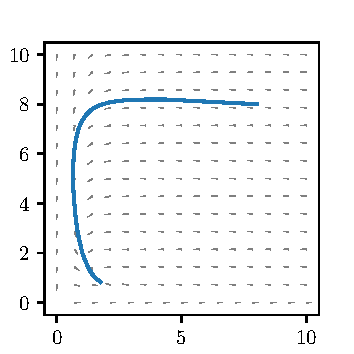
\includegraphics{plots/dynamics.pdf}
\end{figure}
The plot \Cref{fig:dynamics} shows the general phase-portrait and the trajectories of the population dynamics for three different starting points. The dynamics have been stabilized in contrast to the Hopf  bifurcation in the Rosenzweig-MacArthur model under the paradox of enrichment, but the direction of the flow is consistent with the usual Rosenzweig-MacArthur model.
\begin{figure}[H]
  \caption{Pop levels c}
  \label{fig:pop_levels}
  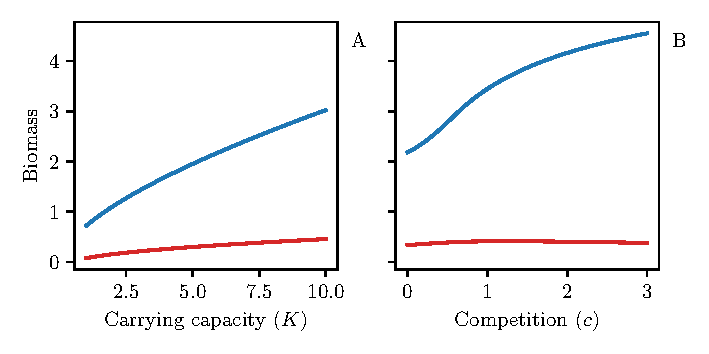
\includegraphics{plots/pop_levels_c.pdf}
\end{figure}
\Cref{fig:pop_levels} reveals how the population levels of consumers and predators change at equilibrium with varying refuge quality (\Cref{fig:pop_levels}(A)), carrying capacity (\Cref{fig:pop_levels}(B)) and intraspecific predator competition (\Cref{fig:pop_levels}(C)).
Increasing the quality of the refuge (\Cref{fig:pop_levels})(A) initially causes an increase in consumer populations (\Cref{fig:pop_levels}(A, blue)) and a decrease in predator populations. The refuge quality reaches a point (\Cref{fig:pop_levels})($q \approx 2.2$)) where the availability of a better refuge causes the population of consumers to go down, presumably since staying in the refuge is individually more advantageous but overall causes lower population levels.

A higher carrying capacity causes higher populations of both consumers and predators populations at equilibrium (\Cref{fig:pop_levels}). The increase in both populations is in contrast to the expected conclusion from the ecosystem exploitation hypothesis, and is probably because the behavioral choice allows the consumers to avoid the risk of predation, while achieving the same fitness.

Varying the intraspecific predator competition causes a decrease in the population of predators (\Cref{fig:pop_levels}(C, red)) until a point where the population stabilizes (\Cref{fig:pop_levels}($c\approx 1/3$)), while the population of consumers continues to increase (\Cref{fig:pop_levels}(C, blue)). The increasing quantity of consumers available must compensate for the intraspecific losses.

\subsubsection*{Spatial distribution}
\begin{figure}[H]
  \caption{Increasing carrying}
  \label{fig:strat_car}
  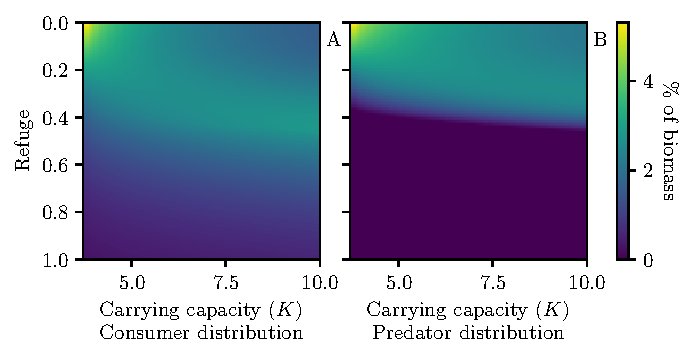
\includegraphics{plots/increasing_car_cap_c.pdf}
\end{figure}
The plots in (\Cref{fig:strat_car}) illustrate the strategies of the consumers (\Cref{fig:strat_car}(A)) and predators (\Cref{fig:strat_car}) at equilibrium when carrying capacity varies. At low carrying capacities, both consumers and predators are relatively spread out, with the peak concentration about halfway to the refuge. As the carrying capacity increases, the distribution becomes more cocentrated and clusters closer to the refuge. The increase in concentration is most marked for the predators. Predators are almost uniformly distributed in the space 0.5-1 at low carrying capacity, while the majority forms a cluster just above the consumer layer at a carrying capacity of 7. Thus the gain from clustering gradually outweighs the loss from the intraspecific predator competition. That both predator and consumer population increase must be the driving factor behind the peak population concentration moving to less productive areas.

A higher carrying capacity leads to more concentrated populations, but the increase in populations leads to greater risk-aversion from the consumers so they concentrate in less desirable zones.

\begin{figure}[H]
  \caption{Increasing competition}
  \label{fig:strat_comp}
    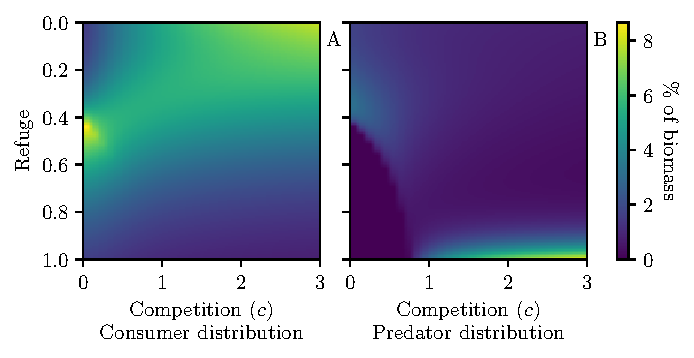
\includegraphics{plots/increasing_competition_c.pdf}
\end{figure}
In \Cref{fig:strat_comp} the intraspecific predator competition is varied and we see the emergent  equilibrium strategy of the consumers (\Cref{fig:strat_comp}(A)) and predators (\Cref{fig:strat_comp}(B)). When there is no intraspecific predator competition, both consumers and predators are highly concentrated at about 0.4. The equilibrium distribution of predators spreads out as we increase the intraspecific predator competition. The previous equilibrium becomes unstable, since the gain from clustering on the consumers is outweighed by the risk of encountering other predators. As the predators gradually spread, it is echoed by the consumers spreading out as well, further incentivicizing predator-spread. When the consumer population spreads out,  the distribution trends towards the more productive layers. Summarizing, highly competitive predators leads to dispersed populations.

\begin{figure}[H]
  \caption{Consumer (A) and predator (B) concentration at equilibrium as a function of changing refuge quality}
  \label{fig:ref_qual}

    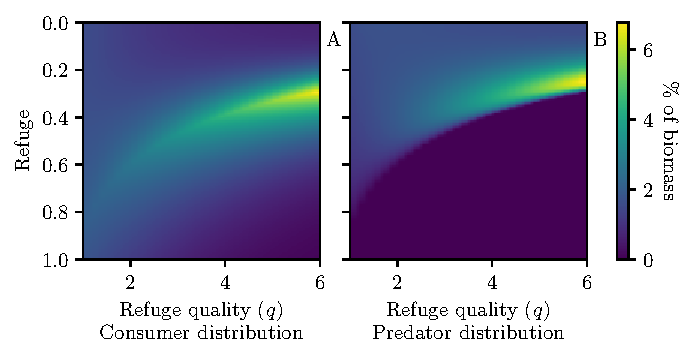
\includegraphics{plots/increasing_refuge_quality_c.pdf}
\end{figure}
\Cref{fig:ref_qual} shows the strategy of consumers (\Cref{fig:ref_qual}(A)) and predators (\Cref{fig:ref_qual}(B)) at equilibrium with varying refuge quality.
